\documentclass[a4paper, 12pt, one column, aas_macros]{article}

%% Language and font encodings. This says how to do hyphenation on end of lines.
\usepackage[english]{babel}
\usepackage[utf8x]{inputenc}
\usepackage[T1]{fontenc}
\usepackage{aas_macros}

%% Sets page size and margins. You can edit this to your liking
\usepackage[top=1.3cm, bottom=2.0cm, outer=2.5cm, inner=2.5cm, heightrounded,
marginparwidth=1.5cm, marginparsep=0.4cm, margin=2.5cm]{geometry}

%% Useful packages
\usepackage{graphicx} %allows you to use jpg or png images. PDF is still recommended
\usepackage[colorlinks=False]{hyperref} % add links inside PDF files
\usepackage{amsmath}  % Math fonts
\usepackage{amsfonts} %
\usepackage{amssymb}  %
\usepackage{array} % enable column sizing
\usepackage[section]{placeins} %prevents figure jumping to end of document
\usepackage{float}
\usepackage[normalem]{ulem}

%% Citation package
\usepackage[authoryear]{natbib}
\bibliographystyle{abbrvnat}
\setcitestyle{authoryear,open={(},close={)}}


\title{NavUP Requirement Summary}
\author{Yacc Group
Josef Alberts
Gregory Austin 
Jocelyn Bondjobo 
Claudio Da Silva        
Thomas Honiball        
Lesego Makaleng       
}

\begin{document}
\maketitle

\begin{abstract}
A Summary regarding Architectural and Systems Design for the NavUP system
\end{abstract}

\section{Use Cases}
\subsubsection{Events}
\textbf{Class Diagram:}
\begin{figure}[H]
\centering
\includegraphics[width=0.8\textwidth]{yacc_team_round_2/images/class/EventsClassDiagram.png}
\caption{Events Class Diagram}
\end{figure}
\textbf{State Diagram:}
\begin{figure}[H]
\centering
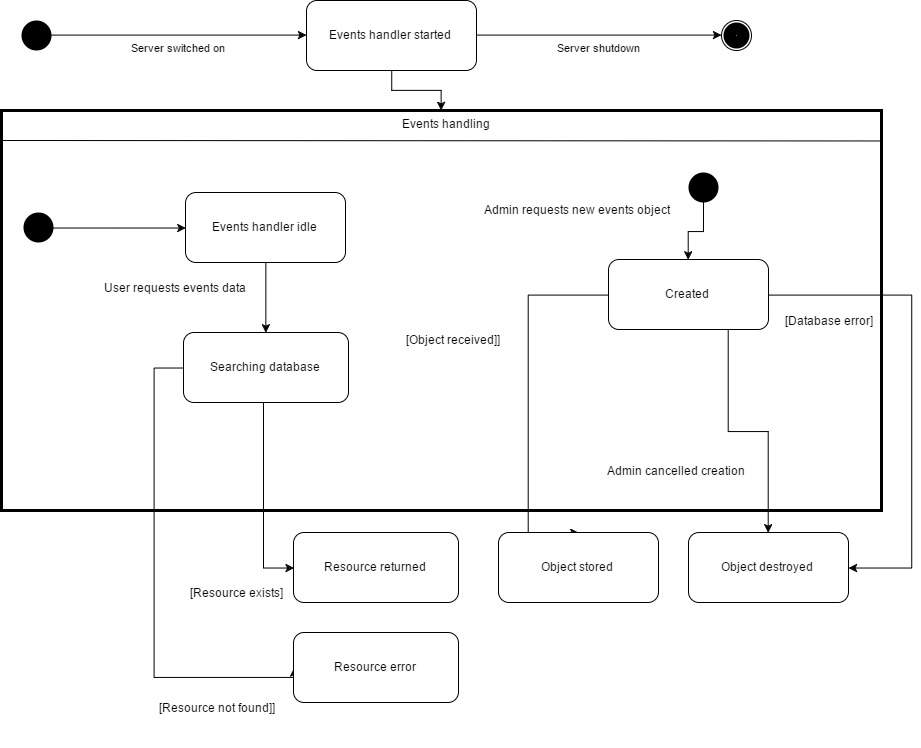
\includegraphics[width=0.8\textwidth]{yacc_team_round_2/images/state/events_state.jpg}
\caption{Events State Diagram}
\end{figure}
\textbf{Sequence Diagram:}
\begin{figure}[H]
\centering
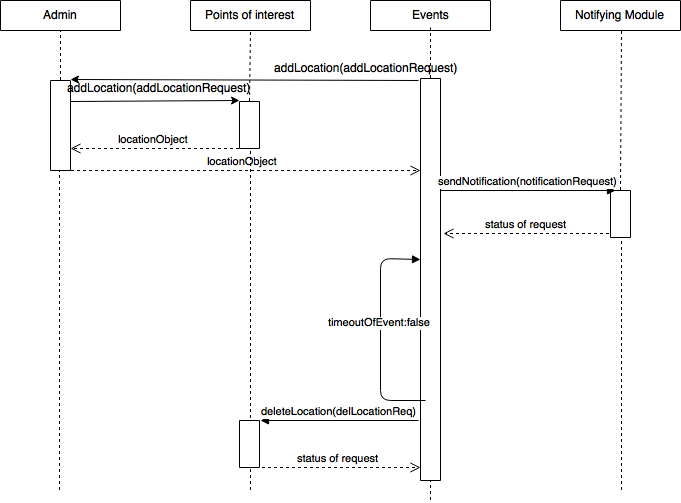
\includegraphics[width=0.8\textwidth]{{yacc_team_round_2/images/sequence/Events sequence diagram}.png}
\caption{Events Sequence Diagram}
\end{figure}

\subsubsection{GIS}
\textbf{Class Diagram:}
\begin{figure}[H]
\centering
\includegraphics[width=0.8\textwidth]{yacc_team_round_2/images/class/GISClassDiagram.png}
\caption{GIS Class Diagram}
\end{figure}
\textbf{State Diagram:}
\begin{figure}[H]
\centering
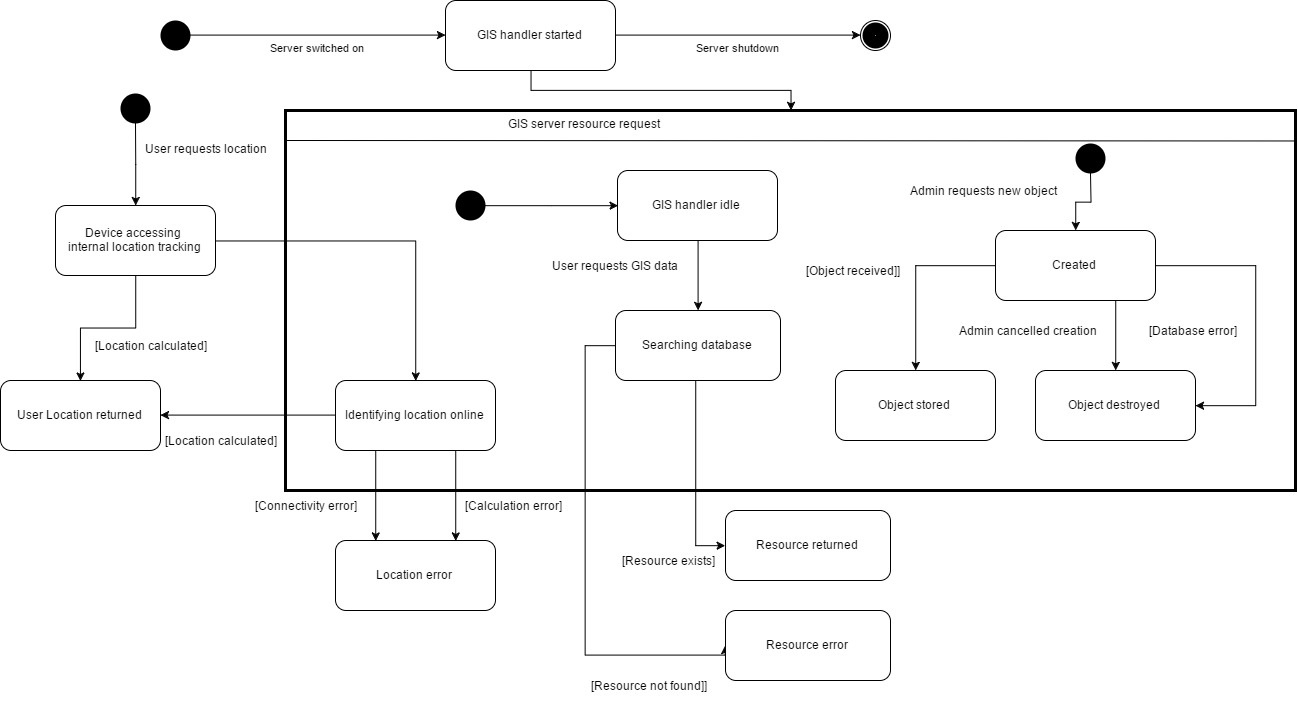
\includegraphics[width=0.8\textwidth]{yacc_team_round_2/images/state/gis_state.jpg}
\caption{GIS State Diagram}
\end{figure}
\textbf{Sequence Diagram:}
\begin{figure}[H]
\centering
\includegraphics[width=0.8\textwidth]{{yacc_team_round_2/images/sequence/GIS Sequence Diagram}.png}
\caption{Events Sequence Diagram}
\end{figure}

\subsubsection{Navigation}
\textbf{Class Diagram:}
\begin{figure}[H]
\centering
\includegraphics[width=0.8\textwidth]{yacc_team_round_2/images/class/EventsClassDiagram.png}
\caption{Events Class Diagram}
\end{figure}
\textbf{State Diagram:}
\begin{figure}[H]
\centering
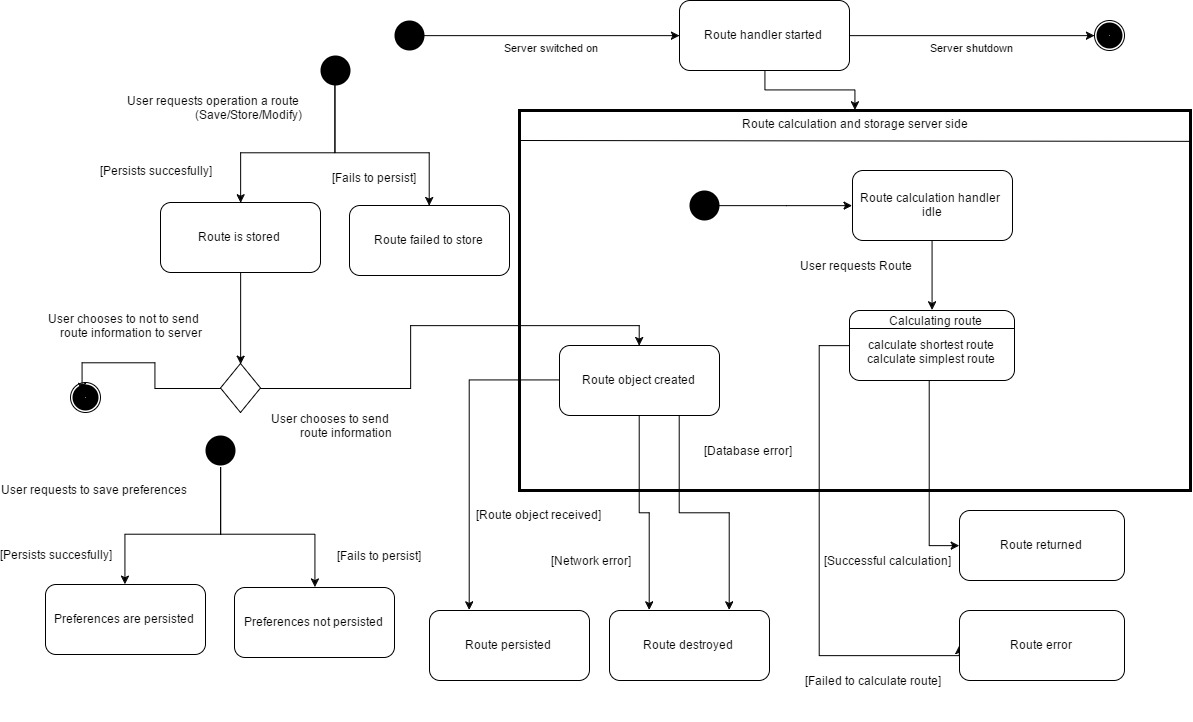
\includegraphics[width=0.8\textwidth]{yacc_team_round_2/images/state/navigation_state.jpg}
\caption{Navigation State Diagram}
\end{figure}
\textbf{Sequence Diagram:}
\begin{figure}[H]
\centering
\includegraphics[width=0.8\textwidth]{{yacc_team_round_2/images/sequence/Navigation Sequence Diagram}.png}
\caption{Navigation Sequence Diagram}
\end{figure}

\subsubsection{Notifications}
\textbf{Class Diagram:}
\begin{figure}[H]
\centering
\includegraphics[width=0.8\textwidth]{yacc_team_round_2/images/class/NotificationsClassDiagram.png}
\caption{Notifications Class Diagram}
\end{figure}
\textbf{State Diagram:}
\begin{figure}[H]
\centering
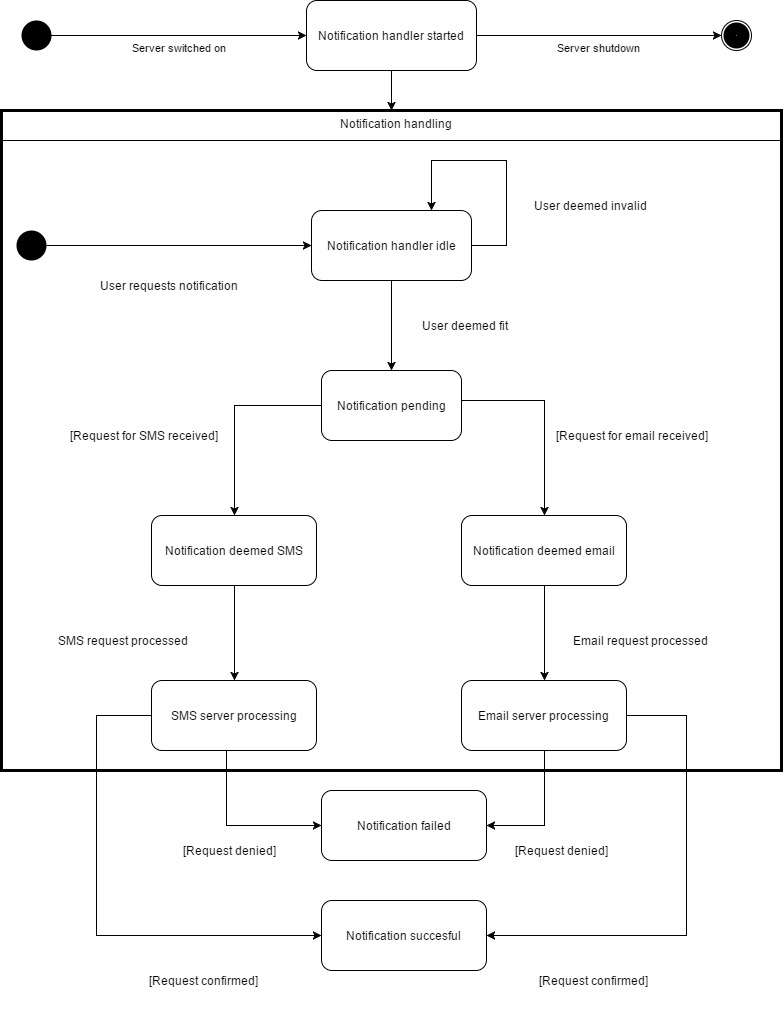
\includegraphics[width=0.8\textwidth]{yacc_team_round_2/images/state/notifications_state.jpg}
\caption{Notifications State Diagram}
\end{figure}
\textbf{Sequence Diagram:}
\begin{figure}[H]
\centering
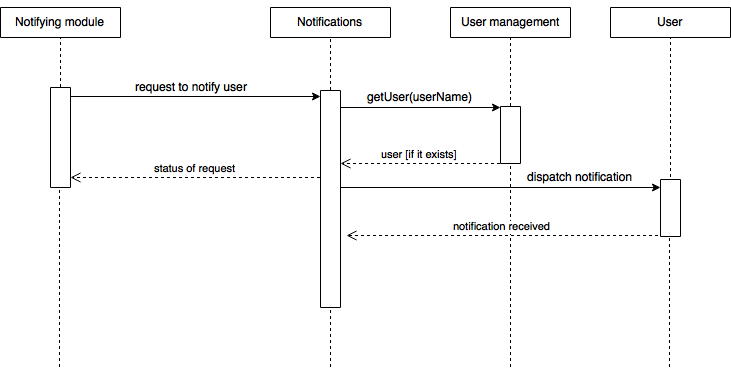
\includegraphics[width=0.8\textwidth]{{yacc_team_round_2/images/sequence/Notification Sequence Diagram}.png}
\caption{Notifications Sequence Diagram}
\end{figure}


\section{Deployment Diagram}

\begin{figure}[H]
\centering
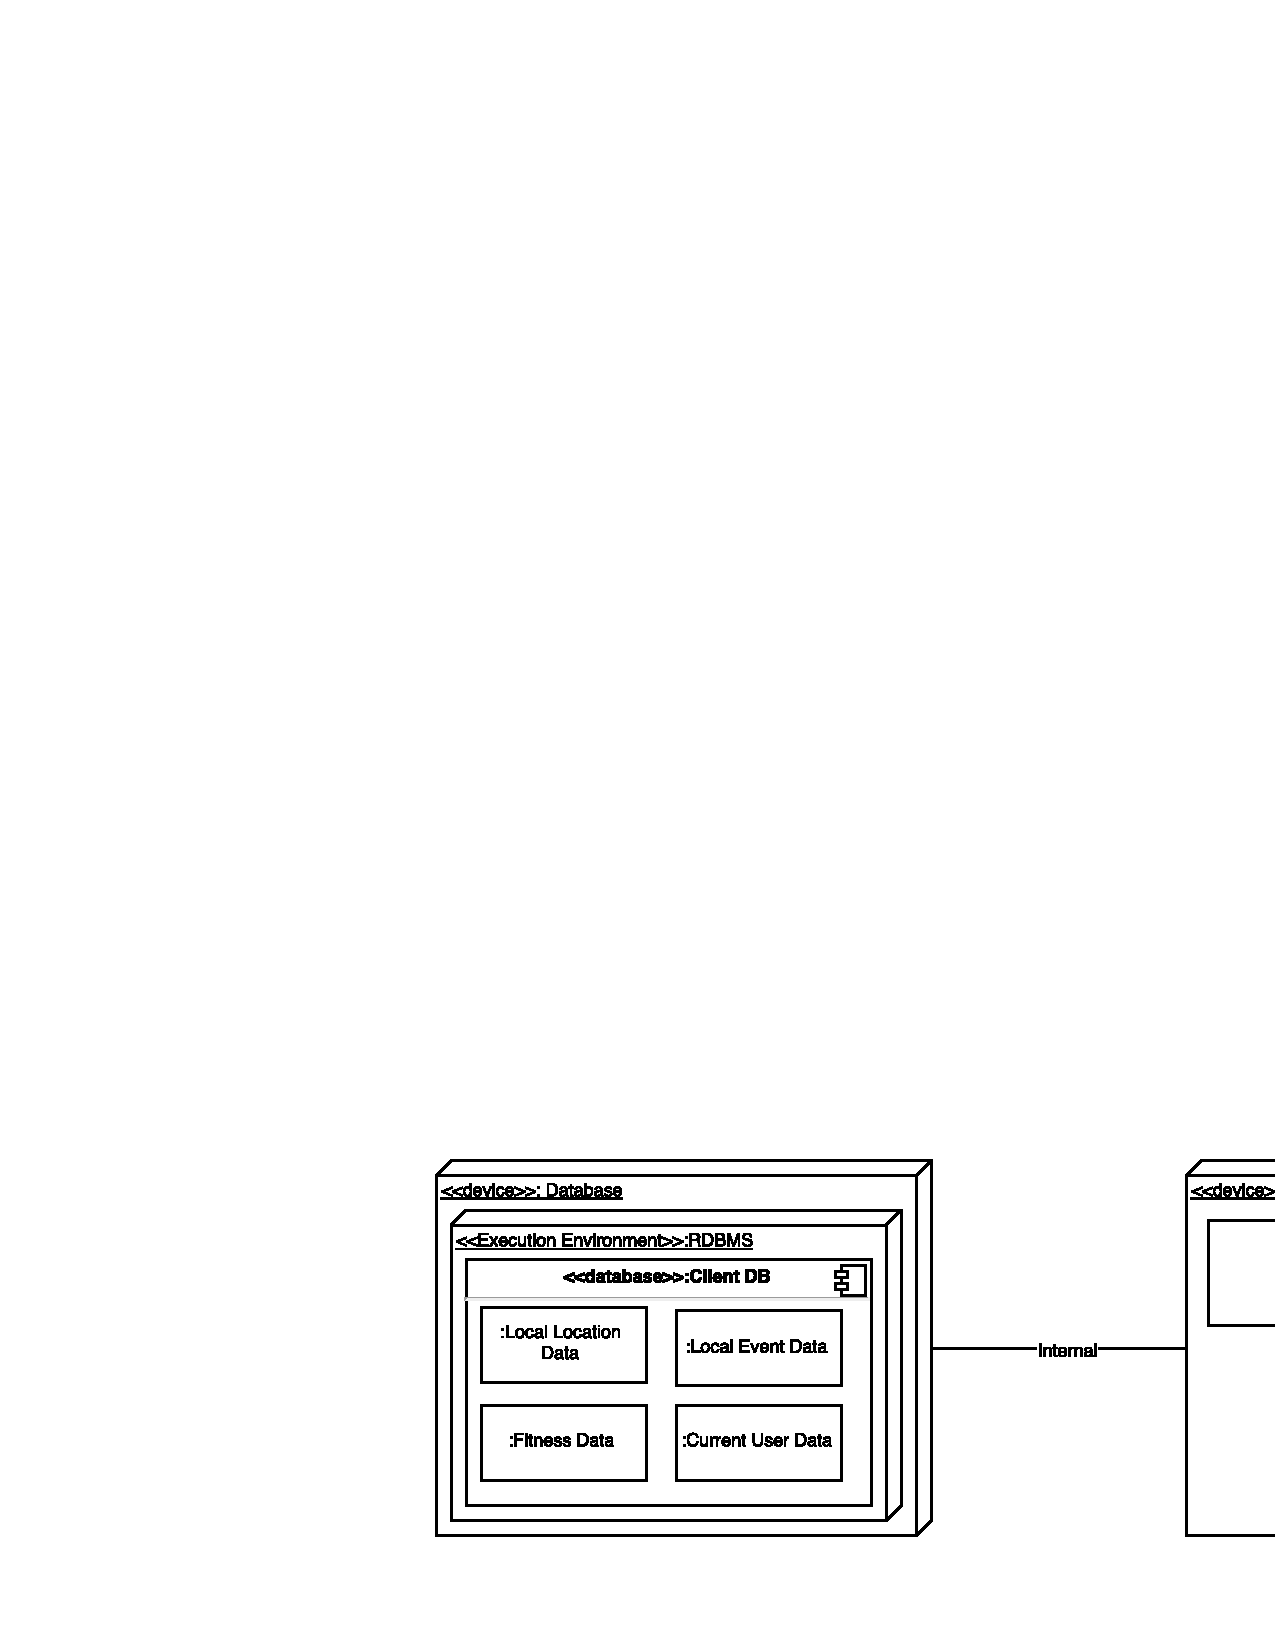
\includegraphics[width=0.8\textwidth]{ {yacc_team_round_2/Deployment Diagram/Deployment Diagram}.pdf }
\caption{NavUP Deployment Diagram}
\end{figure}




\bibliography{refs}
\end{document}
